% from Helmund slides
\documentclass[tikz,border=10pt]{standalone}
%\documentclass[crop, tikz]{standalone}

\usepackage{tikz}

\begin{document}

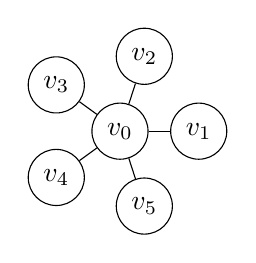
\begin{tikzpicture}
	\tikzstyle{every node} = [draw, shape=circle];
	\node (v0) at (0:    0) {$v_0$};
	\node (v1) at (0:    1) {$v_1$};
	\node (v2) at (72:   1) {$v_2$};
	\node (v3) at (2*72: 1) {$v_3$};
	\node (v4) at (3*72: 1) {$v_4$};	
	\node (v5) at (4*72: 1) {$v_5$};
	
	% draw the edges
	\draw (v0) -- (v1);
	\draw (v0) -- (v2);
	\draw (v0) -- (v3);
	\draw (v0) -- (v4);
	\draw (v0) -- (v5);
\end{tikzpicture}

\end{document}